\chapter{Buffers and Predominance Diagrams}\label{ch:g12:buffers-predominance}

A blood test reports the \omterm{def:g9:acids-bases-ph:ph}{pH} of arterial blood: normally between 7.38 and
7.42. Muscles at work pour acids into the blood, the lungs blow carbon
dioxide out of it, food brings in acids and bases; yet the \omterm{def:g9:acids-bases-ph:ph}{pH} hardly
moves. A pair of species, an acid and its own base, absorbs these shocks.
This chapter shows which form of a couple dominates at a given \omterm{def:g9:acids-bases-ph:ph}{pH}, how a
few drops of a coloured couple reveal the \omterm{def:g9:acids-bases-ph:ph}{pH}, and how a \omterm{def:g6:pure-substances-and-mixtures:mixture}{mixture} of an
acid and its base holds the \omterm{def:g9:acids-bases-ph:ph}{pH} steady.

\begin{recall}
\omterm{def:g12:ka-and-pka:bronsted}{Acid--base couples}, $K_a$ and $pK_a$; the \omterm{def:g9:acids-bases-ph:ph}{pH} of a solution
(\cref{ch:g12:ka-and-pka}, \cref{ch:g9:acids-bases-ph}).
\end{recall}

\begin{omfigure}
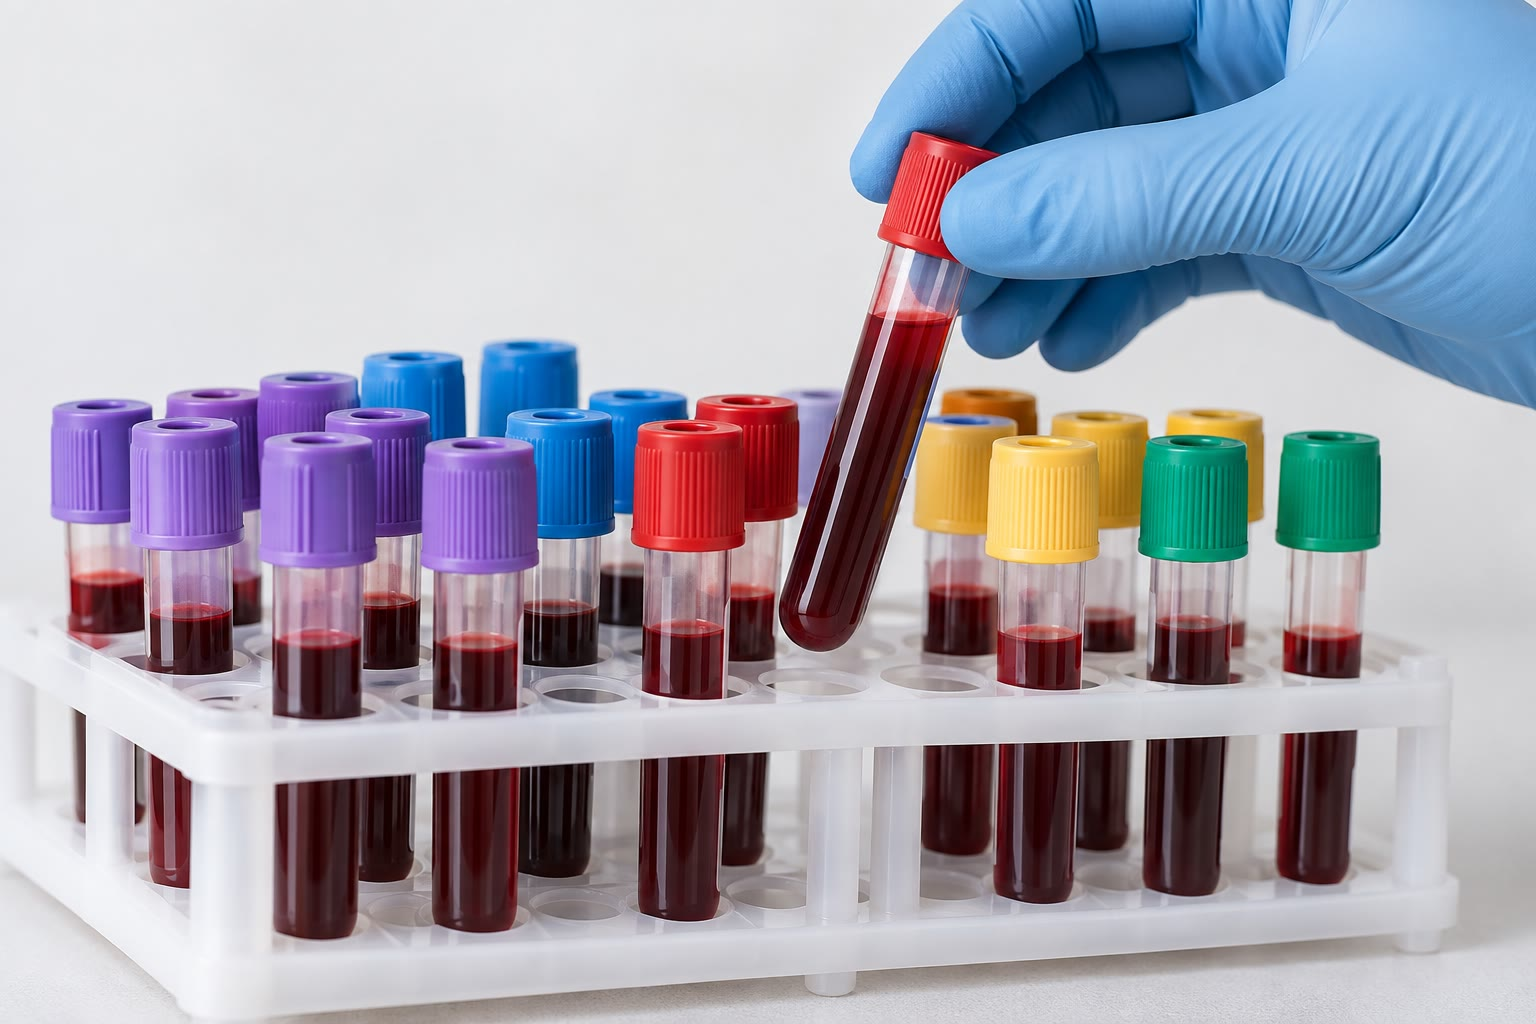
\includegraphics[width=0.45\linewidth]{images/book1/ai/g12-blood-tubes.jpg}

{\small Blood samples: their \omterm{def:g9:acids-bases-ph:ph}{pH} is held within a narrow range.}
\end{omfigure}

\section{Predominance diagrams}

\begin{proposition}[Henderson's relation]\label{prop:g12:buffers-predominance:henderson}
In any \omterm{def:g6:solutions-and-solubility:solute}{aqueous solution} containing the couple \ce{HA}/\ce{A-},
\[
  \mathrm{pH} = pK_a + \log\frac{[\ce{A-}]}{[\ce{HA}]} .
\]
\end{proposition}

\begin{proof}
From $K_a = \dfrac{[\ce{A-}][\ce{H3O+}]}{[\ce{HA}]c^\circ}$, take $-\log$
of both sides: $pK_a = \mathrm{pH} - \log\dfrac{[\ce{A-}]}{[\ce{HA}]}$.
\end{proof}

\begin{definition}[Predominance and distribution diagrams]\label{def:g12:buffers-predominance:predominance}
The \emph{predominance diagram}\index{predominance diagram} of a couple
is a \omterm{def:g9:acids-bases-ph:ph}{pH} axis divided at $pK_a$: below, the acid HA predominates
($[\ce{HA}] > [\ce{A-}]$), above, the base \ce{A-}. The \emph{distribution
diagram}\index{distribution diagram} shows the fraction of each form,
$[\ce{HA}]/c$ and $[\ce{A-}]/c$, against the \omterm{def:g9:acids-bases-ph:ph}{pH}; the two curves cross at
$\mathrm{pH} = pK_a$.
\end{definition}

\begin{method}[Drawing a predominance diagram]\label{met:g12:buffers-predominance:diagram}
\begin{enumerate}
  \item Draw a \omterm{def:g9:acids-bases-ph:ph}{pH} axis from 0 to 14 and mark the $pK_a$ of the couple.
  \item Write the acid to the left of $pK_a$ and the base to the right.
  \item For a species with several couples (an acid with two hydrogens to
        give, an amino acid), mark every $pK_a$: each interval belongs to
        one form.
  \item One unit from $pK_a$, the ratio is already 10 to 1: the minor
        form is under \qty{10}{\percent}.
\end{enumerate}
\end{method}

\begin{omfigure}
\begin{tikzpicture}[font=\small, x=0.62cm]
  % ledger: pka:ethanoic, pka:methanoic, kb:NH3, ka:H2CO3
  \foreach \y/\pk/\acid/\base in {0/3.74/{\ce{HCOOH}}/{\ce{HCOO-}},
      -1.0/4.76/{\ce{CH3COOH}}/{\ce{CH3COO-}}, -2.0/6.37/{\ce{CO2,H2O}}/{\ce{HCO3-}},
      -3.0/9.26/{\ce{NH4+}}/{\ce{NH3}}} {
    \fill[omThm!20] (0,\y) rectangle (\pk,\y+0.5);
    \fill[omDef!20] (\pk,\y) rectangle (14,\y+0.5);
    \draw[black!50] (0,\y) rectangle (14,\y+0.5);
    \node at (\pk/2,\y+0.25) {\acid};
    \node at ({(\pk+14)/2},\y+0.25) {\base};
    \draw[thick] (\pk,\y-0.08) -- (\pk,\y+0.58);
    \node[font=\scriptsize, anchor=south] at (\pk,\y+0.55) {\pk};
  }
  \draw[->] (0,-3.4) -- (14.5,-3.4) node[right] {pH};
  \foreach \k in {0,2,4,6,8,10,12,14} \draw (\k,-3.35) -- (\k,-3.45) node[below, font=\scriptsize] {\k};
\end{tikzpicture}

{\small \omterm{def:g12:buffers-predominance:predominance}{Predominance diagrams} of four couples: the acid (left, red)
dominates below its $pK_a$, the base (right, blue) above.}
\end{omfigure}

\begin{omfigure}
\begin{minipage}{0.49\linewidth}
\begin{tikzpicture}
\begin{axis}[width=\linewidth, height=5cm, xmin=0, xmax=14, ymin=0, ymax=1.05,
    xlabel={pH}, ylabel={fraction}, axis lines*=left, ymajorgrids,
    grid style={gray!20}, tick label style={font=\scriptsize},
    label style={font=\small}, title={\small ethanoic acid},
    title style={yshift=-4pt}]
  \addplot[very thick, omThm] table[x=pH, y=HA] {figdata/out/grade-12-buffers-predominance-a.dat};
  \addplot[very thick, omDef] table[x=pH, y=A] {figdata/out/grade-12-buffers-predominance-a.dat};
  \addplot[dashed, black!50] coordinates {(4.76,0) (4.76,1)};
  \node[font=\scriptsize, omThm] at (axis cs:2.2,0.85) {\ce{CH3COOH}};
  \node[font=\scriptsize, omDef] at (axis cs:7.6,0.85) {\ce{CH3COO-}};
\end{axis}
\end{tikzpicture}
\end{minipage}\hfill
\begin{minipage}{0.49\linewidth}
\begin{tikzpicture}
\begin{axis}[width=\linewidth, height=5cm, xmin=0, xmax=14, ymin=0, ymax=1.05,
    xlabel={pH}, ylabel={fraction}, axis lines*=left, ymajorgrids,
    grid style={gray!20}, tick label style={font=\scriptsize},
    label style={font=\small}, title={\small glycine},
    title style={yshift=-4pt}]
  \addplot[very thick, omThm] table[x=pH, y=cation] {figdata/out/grade-12-buffers-predominance-b.dat};
  \addplot[very thick, omMeth] table[x=pH, y=zwitterion] {figdata/out/grade-12-buffers-predominance-b.dat};
  \addplot[very thick, omDef] table[x=pH, y=anion] {figdata/out/grade-12-buffers-predominance-b.dat};
  \node[font=\scriptsize, omThm] at (axis cs:1.0,0.55) {cation};
  \node[font=\scriptsize, omMeth] at (axis cs:6.1,0.88) {zwitterion};
  \node[font=\scriptsize, omDef] at (axis cs:12.6,0.55) {anion};
\end{axis}
\end{tikzpicture}
\end{minipage}

{\small \omterm{def:g12:buffers-predominance:predominance}{Distribution diagrams}, computed from the $pK_a$ values. Left:
ethanoic acid, the curves cross at 4.76. Right: glycine,
\ce{H2N-CH2-COOH}, with two couples ($pK_a$ 2.35 and 9.78): the \omterm{def:g9:ions:ion}{cation}
\ce{H3N+-CH2-COOH}, the zwitterion \ce{H3N+-CH2-COO-} and the \omterm{def:g9:ions:ion}{anion}
\ce{H2N-CH2-COO-}.}
\end{omfigure}

\begin{example}[Glycine in the body]\label{ex:g12:buffers-predominance:glycine}
% ledger: pka:glycine1, pka:glycine2, ph:blood
At the \omterm{def:g9:acids-bases-ph:ph}{pH} of blood, about 7.4, glycine lies between its two $pK_a$
values: it is almost entirely in the zwitterion form, carrying a
positive charge on its nitrogen and a negative charge on its carboxylate,
neutral overall. Every amino acid behaves the same way.
\end{example}

\section{Acid--base indicators}


\begin{definition}[Acid--base indicator, colour-change range]\label{def:g12:buffers-predominance:indicator}
An \emph{acid--base indicator}\index{acid--base indicator} is a couple
\ce{HInd}/\ce{Ind-} whose two forms have different colours, used in very
small amounts. Its \emph{colour-change range}\index{colour-change range}
is the \omterm{def:g9:acids-bases-ph:ph}{pH} interval over which the colour is seen to change, roughly
$pK_a - 1$ to $pK_a + 1$: below, the colour of \ce{HInd} is seen, above,
that of \ce{Ind-}, and in between a \omterm{def:g6:pure-substances-and-mixtures:mixture}{mixture} of the two.
\end{definition}

\begin{omfigure}
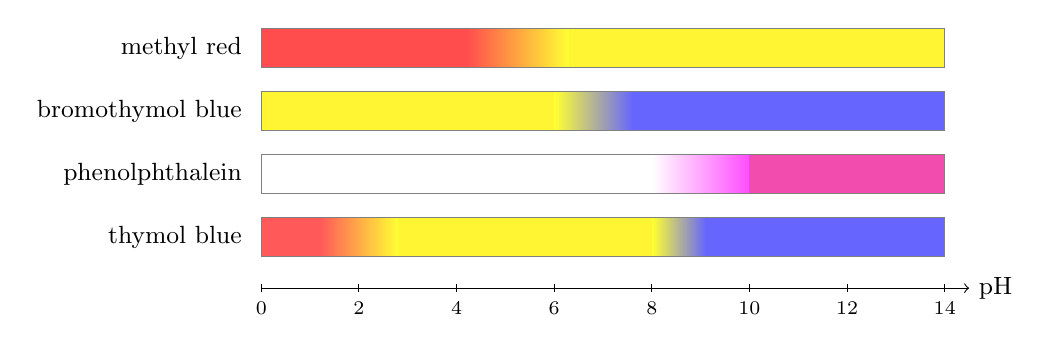
\begin{tikzpicture}[font=\small, x=0.62cm]
  % ledger: ind:methyl-red, ind:BBT, ind:phenolphthalein, ind:thymol-blue, ind:range-rule
  \foreach \y/\name/\a/\b/\ca/\cm/\cb in {
      0/{methyl red}/4.2/6.3/red!70/orange/yellow!80,
      -0.8/{bromothymol blue}/6.0/7.6/yellow!80/green!60/blue!60,
      -1.6/{phenolphthalein}/8.0/10.0/white/magenta!25/magenta!70} {
    \fill[\ca] (0,\y) rectangle (\a,\y+0.5);
    \shade[left color=\ca, right color=\cb] (\a,\y) rectangle (\b,\y+0.5);
    \fill[\cb] (\b,\y) rectangle (14,\y+0.5);
    \draw[black!50] (0,\y) rectangle (14,\y+0.5);
    \node[anchor=east] at (-0.2,\y+0.25) {\name};
  }
  \fill[red!65] (0,-2.4) rectangle (1.2,-1.9);
  \shade[left color=red!65, right color=yellow!80] (1.2,-2.4) rectangle (2.8,-1.9);
  \fill[yellow!80] (2.8,-2.4) rectangle (8.0,-1.9);
  \shade[left color=yellow!80, right color=blue!60] (8.0,-2.4) rectangle (9.1,-1.9);
  \fill[blue!60] (9.1,-2.4) rectangle (14,-1.9);
  \draw[black!50] (0,-2.4) rectangle (14,-1.9);
  \node[anchor=east] at (-0.2,-2.15) {thymol blue};
  \draw[->] (0,-2.8) -- (14.5,-2.8) node[right] {pH};
  \foreach \k in {0,2,4,6,8,10,12,14} \draw (\k,-2.75) -- (\k,-2.85) node[below, font=\scriptsize] {\k};
\end{tikzpicture}

{\small Colours of four indicators against the \omterm{def:g9:acids-bases-ph:ph}{pH}; the shaded parts are
the \omterm{def:g12:buffers-predominance:indicator}{colour-change ranges}. Thymol blue, with two couples, has two
ranges.}
\end{omfigure}

\begin{method}[Choosing an indicator]\label{met:g12:buffers-predominance:indicator}
To detect when a solution passes a given \omterm{def:g9:acids-bases-ph:ph}{pH} (the \omterm{def:g9:acids-bases-ph:ph}{pH} at the end of a
\omterm{def:g11:titration:titration}{titration}, for example), choose an indicator whose \omterm{def:g12:buffers-predominance:indicator}{colour-change range}
contains that \omterm{def:g9:acids-bases-ph:ph}{pH}: the colour then changes exactly there.
\end{method}

\section{Buffer solutions}

\begin{definition}[Buffer solution]\label{def:g12:buffers-predominance:buffer}
A \emph{buffer solution}\index{buffer solution} is a solution whose \omterm{def:g9:acids-bases-ph:ph}{pH}
changes very little when a little acid or base is added, or when it is
diluted. It is usually made of a \omterm{def:g12:ka-and-pka:strong-acid}{weak acid} and its conjugate base in
comparable amounts; its \omterm{def:g9:acids-bases-ph:ph}{pH} is then close to the $pK_a$ of the couple.
\end{definition}

\begin{proposition}[Why a buffer resists]\label{prop:g12:buffers-predominance:buffer}
In a buffer of \ce{HA} and \ce{A-}, an added \omterm{def:g12:ka-and-pka:strong-acid}{strong acid} is consumed by
\ce{A-} (\ce{A- + H3O+ -> HA + H2O}) and an added \omterm{def:g12:ka-and-pka:strong-acid}{strong base} by \ce{HA}
(\ce{HA + OH- -> A- + H2O}); the ratio $[\ce{A-}]/[\ce{HA}]$, and so the
\omterm{def:g9:acids-bases-ph:ph}{pH}, changes only a little. \omterm{def:g10:concentration-and-dilution:dilution}{Dilution} does not change the ratio at all.
\end{proposition}

\begin{proof}
By Henderson's relation the \omterm{def:g9:acids-bases-ph:ph}{pH} depends only on the ratio. Adding
\qty{1}{mmol} of acid to a buffer holding \qty{10}{mmol} of each form
changes the ratio from $10/10$ to $9/11$, and the \omterm{def:g9:acids-bases-ph:ph}{pH} by
$\log(9/11) = -0.09$ only.
\end{proof}

\begin{omfigure}
\begin{tikzpicture}
\begin{axis}[width=0.75\linewidth, height=5.6cm, xmin=0, xmax=10, ymin=0,
    ymax=8, xlabel={\ce{HCl} at \qty{0.10}{mol/L} added (\si{mL})},
    ylabel={pH}, axis lines*=left, ymajorgrids, grid style={gray!20},
    tick label style={font=\small}, label style={font=\small},
    legend style={font=\small, at={(0.98,0.97)}, anchor=north east,
    draw=none, fill=white}, legend cell align=left]
  % ledger: pka:ethanoic (buffer recipe: exercise data)
  \addplot[very thick, omThm, mark=*, mark size=1.3pt] table[x=V, y=water]
    {figdata/out/grade-12-buffers-predominance-c.dat};
  \addplot[very thick, omDef, mark=*, mark size=1.3pt] table[x=V, y=buffer]
    {figdata/out/grade-12-buffers-predominance-c.dat};
  \legend{\qty{100}{mL} of pure water, \qty{100}{mL} of ethanoate buffer}
\end{axis}
\end{tikzpicture}

{\small Adding hydrochloric acid to pure water and to a buffer of
ethanoic acid and sodium ethanoate (\qty{0.10}{mol/L} each). The \omterm{def:g9:acids-bases-ph:ph}{pH} of
water falls from 7 to about 2; that of the buffer from 4.76 to 4.67.}
\end{omfigure}

\begin{method}[Preparing a buffer]\label{met:g12:buffers-predominance:prepare}
\begin{enumerate}
  \item Choose a couple whose $pK_a$ is within one unit of the \omterm{def:g9:acids-bases-ph:ph}{pH} wanted
        (ideally close to it).
  \item Compute the ratio $[\ce{A-}]/[\ce{HA}] = 10^{\mathrm{pH} - pK_a}$.
  \item \omterm{def:g2:mixing-and-dissolving:mix}{Mix} the \omterm{def:g12:ka-and-pka:strong-acid}{weak acid} and a salt of its base in that ratio, at
        concentrations high enough for the amounts of acid or base to be
        absorbed.
\end{enumerate}
\end{method}

\begin{inthelab}[Preparing a buffer at pH 4.8]
\qty{50.0}{mL} of ethanoic acid at \qty{0.10}{mol/L} are mixed with
\qty{50.0}{mL} of sodium ethanoate at \qty{0.10}{mol/L}; a \omterm{def:g9:acids-bases-ph:ph-paper}{pH meter} reads
about 4.8. A few drops of hydrochloric acid at \qty{1}{mol/L} barely move
the reading, while the same drops in \qty{100}{mL} of distilled water
bring it down to about 3.
\end{inthelab}

\section{Buffers in living things}

\begin{example}[The blood's buffer]\label{ex:g12:buffers-predominance:blood}
% ledger: pk:blood-bicarb, ph:blood, hco3:blood
The main buffer of blood is the couple of dissolved carbon dioxide and
the hydrogencarbonate \omterm{def:g9:ions:ion}{ion}, \ce{CO2,H2O}/\ce{HCO3-}. In blood, the
physiologists use for it the relation $\mathrm{pH} = 6.1 +
\log\big([\ce{HCO3-}]/[\ce{CO2}]\big)$. The lungs remove carbon dioxide,
the kidneys adjust the hydrogencarbonate: together they hold the ratio,
and so the \omterm{def:g9:acids-bases-ph:ph}{pH}.
\end{example}

\begin{omfigure}
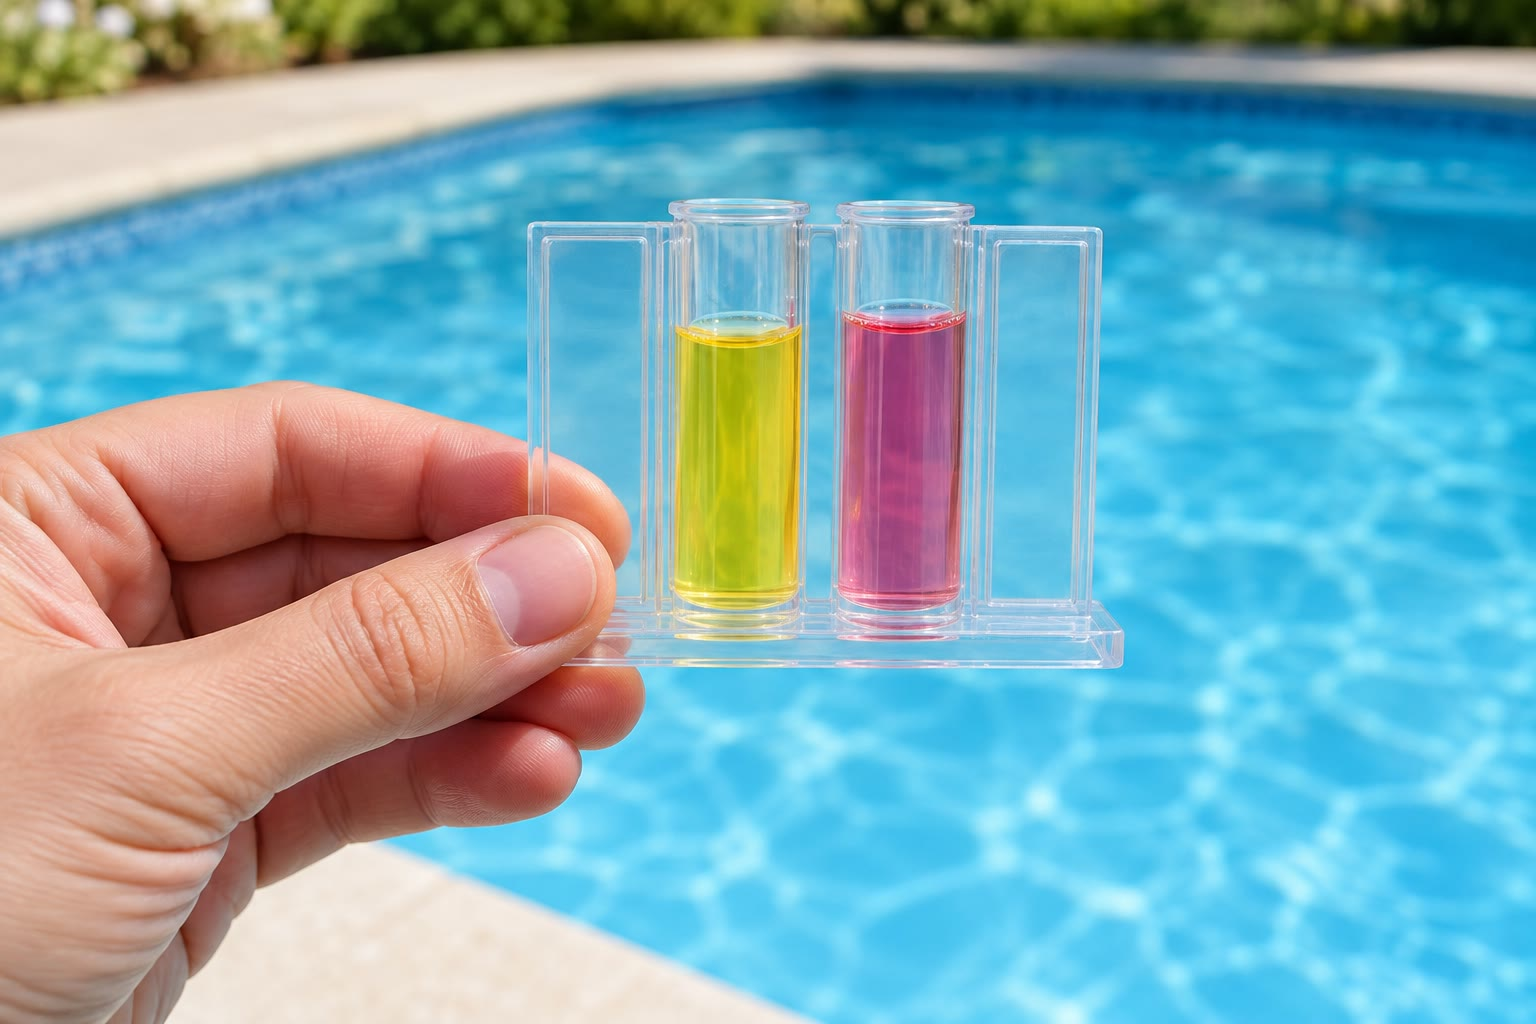
\includegraphics[width=0.45\linewidth]{images/book1/ai/g12-pool-test.jpg}

{\small Testing swimming-pool water: the colours of indicators give the
\omterm{def:g9:acids-bases-ph:ph}{pH}.}
\end{omfigure}

\section{Exercises}


\begin{exercise}[$\star$]\label{exo:g12:buffers-predominance:1}
Which form of the couple \ce{CH3COOH}/\ce{CH3COO-} ($pK_a = 4.76$)
predominates at \omterm{def:g9:acids-bases-ph:ph}{pH} 2, at \omterm{def:g9:acids-bases-ph:ph}{pH} 4.76 and at \omterm{def:g9:acids-bases-ph:ph}{pH} 7?
\end{exercise}

\begin{exercise}[$\star$]\label{exo:g12:buffers-predominance:2}
On the \omterm{def:g12:buffers-predominance:predominance}{distribution diagram} of ethanoic acid, read the fraction of
\ce{CH3COO-} at \omterm{def:g9:acids-bases-ph:ph}{pH} 4 and at \omterm{def:g9:acids-bases-ph:ph}{pH} 6.
\end{exercise}

\begin{exercise}[$\star$]\label{exo:g12:buffers-predominance:3}
What colour does bromothymol blue show at \omterm{def:g9:acids-bases-ph:ph}{pH} 5? At \omterm{def:g9:acids-bases-ph:ph}{pH} 7? At \omterm{def:g9:acids-bases-ph:ph}{pH} 9?
\end{exercise}

\begin{exercise}[$\star$]\label{exo:g12:buffers-predominance:4}
Which form of the couple \ce{NH4+}/\ce{NH3} predominates in a solution at
\omterm{def:g9:acids-bases-ph:ph}{pH} 7.4? At \omterm{def:g9:acids-bases-ph:ph}{pH} 11?
\end{exercise}

\begin{exercise}[$\star$]\label{exo:g12:buffers-predominance:5}
Why are indicators used in very small amounts?
\end{exercise}

\begin{exercise}[$\star\star$]\label{exo:g12:buffers-predominance:6}
Compute the ratio $[\ce{CH3COO-}]/[\ce{CH3COOH}]$ at \omterm{def:g9:acids-bases-ph:ph}{pH} 3.76, 4.76 and
5.76.
\end{exercise}

\begin{exercise}[$\star\star$]\label{exo:g12:buffers-predominance:7}
A \omterm{def:g11:titration:titration}{titration} ends at \omterm{def:g9:acids-bases-ph:ph}{pH} 8.7. Which of the four indicators of the figure
would you choose? Why not methyl red?
\end{exercise}

\begin{exercise}[$\star\star$]\label{exo:g12:buffers-predominance:8}
A buffer contains \qty{0.20}{mol/L} of ethanoic acid and
\qty{0.10}{mol/L} of sodium ethanoate. Compute its \omterm{def:g9:acids-bases-ph:ph}{pH}.
\end{exercise}

\begin{exercise}[$\star\star$]\label{exo:g12:buffers-predominance:9}
Using the glycine diagram, give the predominant form at \omterm{def:g9:acids-bases-ph:ph}{pH} 1, 6 and 12,
with its charge.
\end{exercise}

\begin{exercise}[$\star\star$]\label{exo:g12:buffers-predominance:10}
Read the response curves: by how much does the \omterm{def:g9:acids-bases-ph:ph}{pH} of water fall after
\qty{1.0}{mL} of acid? And that of the buffer?
\end{exercise}

\begin{exercise}[$\star\star$]\label{exo:g12:buffers-predominance:11}
Which couple of the predominance figure would you choose to make a
buffer at \omterm{def:g9:acids-bases-ph:ph}{pH} 9.5? In what ratio would you \omterm{def:g2:mixing-and-dissolving:mix}{mix} its two forms?
\end{exercise}

\begin{exercise}[$\star\star\star$]\label{exo:g12:buffers-predominance:12}
The ethanoate buffer of the figure (\qty{10}{mmol} of each form) receives
hydrochloric acid. How much acid can it take before its \omterm{def:g9:acids-bases-ph:ph}{pH} has fallen by
one unit? Why is a more concentrated buffer said to have a larger
capacity?
\end{exercise}

\begin{exercise}[$\star\star\star$]\label{exo:g12:buffers-predominance:13}
What volume of sodium ethanoate solution at \qty{0.10}{mol/L} must be
added to \qty{100}{mL} of ethanoic acid at \qty{0.10}{mol/L} to obtain a
buffer at \omterm{def:g9:acids-bases-ph:ph}{pH} 5.0?
\end{exercise}

\begin{exercise}[$\star\star\star$]\label{exo:g12:buffers-predominance:14}
Thymol blue has two \omterm{def:g12:buffers-predominance:indicator}{colour-change ranges}. Explain why, and give its
colour at \omterm{def:g9:acids-bases-ph:ph}{pH} 1, 5 and 10.
\end{exercise}

\begin{exercise}[$\star\star\star$]\label{exo:g12:buffers-predominance:15}
A buffer at \omterm{def:g9:acids-bases-ph:ph}{pH} 4.76 is diluted ten times with distilled water. What is
its new \omterm{def:g9:acids-bases-ph:ph}{pH}, according to Henderson's relation? What happens if a \omterm{def:g12:ka-and-pka:strong-acid}{strong
acid} of the same \omterm{def:g9:acids-bases-ph:ph}{pH} is diluted ten times?
\end{exercise}

\section{Problem: Blood's Buffer}

\begin{problem}[{Weekend problem --- what ratio of hydrogencarbonate to
carbon dioxide keeps blood at pH 7.4?}]
\label{pb:g12:buffers-predominance:1}
% ledger: pk:blood-bicarb, ph:blood, hco3:blood
The \omterm{def:g9:acids-bases-ph:ph}{pH} of arterial blood is normally between 7.38 and 7.42. Its main
buffer is the couple \ce{CO2,H2O}/\ce{HCO3-}, for which physiologists use
$\mathrm{pH} = 6.1 + \log\big([\ce{HCO3-}]/[\ce{CO2}]\big)$. The normal
hydrogencarbonate concentration of blood is 22 to \qty{28}{mmol/L}.

\medskip
\noindent\textbf{Part I --- The couple.}
\begin{enumerate}
  \item Write the reaction of dissolved carbon dioxide with water that
        gives hydrogencarbonate \omterm{def:g9:ions:ion}{ions}.
  \item Which species is the acid, which the base?
  \item The value 6.1 differs from the 6.37 of the table of $pK_a$. Give a
        reason (think of the temperature of the body and of the other
        \omterm{def:g9:ions:ion}{ions} present).
  \item What amount of hydrogencarbonate do \qty{5.0}{L} of blood hold
        at \qty{24}{mmol/L}?
\end{enumerate}

\medskip
\noindent\textbf{Part II --- Predominance.}
\begin{enumerate}[resume]
  \item Draw the \omterm{def:g12:buffers-predominance:predominance}{predominance diagram} of the couple with $pK = 6.1$.
  \item Which form predominates in blood?
  \item Is blood slightly acidic or slightly basic?
\end{enumerate}

\medskip
\noindent\textbf{Part III --- The ratio.}
\begin{enumerate}[resume]
  \item Using the relation, compute the ratio $[\ce{HCO3-}]/[\ce{CO2}]$
        at \omterm{def:g9:acids-bases-ph:ph}{pH} 7.4.
  \item With $[\ce{HCO3-}] = \qty{24}{mmol/L}$, compute $[\ce{CO2}]$.
  \item Compute the ratio at the two ends of the normal range, 7.38 and
        7.42.
  \item What fraction of the couple is in the hydrogencarbonate form at
        \omterm{def:g9:acids-bases-ph:ph}{pH} 7.4?
  \item Blood that is too basic may reach \omterm{def:g9:acids-bases-ph:ph}{pH} 7.6. What is the ratio
        then?
\end{enumerate}

\medskip
\noindent\textbf{Part IV --- When the balance is lost.}
\begin{enumerate}[resume]
  \item During intense effort, acids enter the blood. Which form of the
        couple consumes them? Write the reaction.
  \item If the \omterm{def:g9:acids-bases-ph:ph}{pH} fell to 7.1, what would the ratio become?
  \item With unchanged hydrogencarbonate, how much would the carbon
        dioxide have to increase? What do the lungs do to fight back?
  \item Why is a \omterm{def:g12:ka-and-pka:strong-acid}{weak acid} with its base, rather than a \omterm{def:g12:ka-and-pka:strong-acid}{strong acid}, the
        right tool to hold a \omterm{def:g9:acids-bases-ph:ph}{pH}?
  \item By how much does the \omterm{def:g9:acids-bases-ph:ph}{pH} change if both concentrations are divided
        by two? Why?
  \item State the final answer: what is the hydrogencarbonate to carbon
        dioxide ratio of blood at \omterm{def:g9:acids-bases-ph:ph}{pH} 7.4?
\end{enumerate}
\end{problem}
